\icode{E-MD-SI-L2-261114-007}
如图所示，在竖直平面内有一矩形，其长边与一圆的底部相切于 \(O\) 点，现在有三条光滑轨道 \(a\)、\(b\)、\(c\)，它们的上端位于圆周上，下端在矩形的底边，三轨道都经过切点 \(O\)。现在让一物块先后从三轨道顶端由静止下滑至底端（轨道先后放置），则物块在每一条倾斜轨道上滑动时所经历的时间关系为\paren[]
	
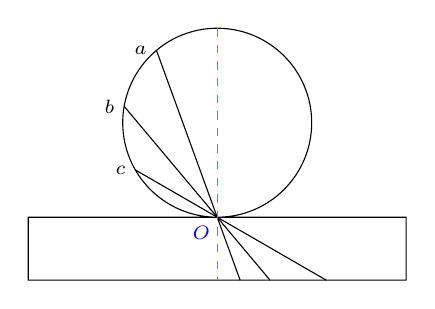
\begin{tikzpicture}[font=\scriptsize]
	\draw (0,1.2) circle(1.2) (-2.4,0) rectangle(2.4,-.8);
	\foreach \angle/\c in {20/a,40/b,60/c}
		\draw (0,0)--({90+\angle}:{2.4*cos(\angle)})node[left]{\(\c\)} (0,0)--({-90+\angle}:{.8/cos(\angle)});
	\draw[dashed,cyan] (0,2.4)--(0,-.8);
	\node at(-.2,-.2)[blue]{\(O\)};
\end{tikzpicture}
\begin{choices}
	\item \(t_a > t_b > t_c\)
	\item \(t_a < t_b < t_c\)
	\item \(t_a = t_b = t_c\)
	\item 无法确定
\end{choices}
\begin{answer}
    A\qquad 提示：
\end{answer}